
%% bare_jrnl.tex
%% V1.3
%% 2007/01/11
%% by Michael Shell
%% see http://www.michaelshell.org/
%% for current contact information.
%%
%% This is a skeleton file demonstrating the use of IEEEtran.cls
%% (requires IEEEtran.cls version 1.7 or later) with an IEEE journal paper.
%%
%% Support sites:
%% http://www.michaelshell.org/tex/ieeetran/
%% http://www.ctan.org/tex-archive/macros/latex/contrib/IEEEtran/
%% and
%% http://www.ieee.org/



% *** Authors should verify (and, if needed, correct) their LaTeX system  ***
% *** with the testflow diagnostic prior to trusting their LaTeX platform ***
% *** with production work. IEEE's font choices can trigger bugs that do  ***
% *** not appear when using other class files.                            ***
% The testflow support page is at:
% http://www.michaelshell.org/tex/testflow/


%%*************************************************************************
%% Legal Notice:
%% This code is offered as-is without any warranty either expressed or
%% implied; without even the implied warranty of MERCHANTABILITY or
%% FITNESS FOR A PARTICULAR PURPOSE! 
%% User assumes all risk.
%% In no event shall IEEE or any contributor to this code be liable for
%% any damages or losses, including, but not limited to, incidental,
%% consequential, or any other damages, resulting from the use or misuse
%% of any information contained here.
%%
%% All comments are the opinions of their respective authors and are not
%% necessarily endorsed by the IEEE.
%%
%% This work is distributed under the LaTeX Project Public License (LPPL)
%% ( http://www.latex-project.org/ ) version 1.3, and may be freely used,
%% distributed and modified. A copy of the LPPL, version 1.3, is included
%% in the base LaTeX documentation of all distributions of LaTeX released
%% 2003/12/01 or later.
%% Retain all contribution notices and credits.
%% ** Modified files should be clearly indicated as such, including  **
%% ** renaming them and changing author support contact information. **
%%
%% File list of work: IEEEtran.cls, IEEEtran_HOWTO.pdf, bare_adv.tex,
%%                    bare_conf.tex, bare_jrnl.tex, bare_jrnl_compsoc.tex
%%*************************************************************************

% Note that the a4paper option is mainly intended so that authors in
% countries using A4 can easily print to A4 and see how their papers will
% look in print - the typesetting of the document will not typically be
% affected with changes in paper size (but the bottom and side margins will).
% Use the testflow package mentioned above to verify correct handling of
% both paper sizes by the user's LaTeX system.
%
% Also note that the "draftcls" or "draftclsnofoot", not "draft", option
% should be used if it is desired that the figures are to be displayed in
% draft mode.
%
\documentclass[journal]{IEEEtran}
\usepackage{blindtext}
\usepackage{graphicx}

% Some very useful LaTeX packages include:
% (uncomment the ones you want to load)


% *** MISC UTILITY PACKAGES ***
%
%\usepackage{ifpdf}
% Heiko Oberdiek's ifpdf.sty is very useful if you need conditional
% compilation based on whether the output is pdf or dvi.
% usage:
% \ifpdf
%   % pdf code
% \else
%   % dvi code
% \fi
% The latest version of ifpdf.sty can be obtained from:
% http://www.ctan.org/tex-archive/macros/latex/contrib/oberdiek/
% Also, note that IEEEtran.cls V1.7 and later provides a builtin
% \ifCLASSINFOpdf conditional that works the same way.
% When switching from latex to pdflatex and vice-versa, the compiler may
% have to be run twice to clear warning/error messages.






% *** CITATION PACKAGES ***
%
%\usepackage{cite}
% cite.sty was written by Donald Arseneau
% V1.6 and later of IEEEtran pre-defines the format of the cite.sty package
% \cite{} output to follow that of IEEE. Loading the cite package will
% result in citation numbers being automatically sorted and properly
% "compressed/ranged". e.g., [1], [9], [2], [7], [5], [6] without using
% cite.sty will become [1], [2], [5]--[7], [9] using cite.sty. cite.sty's
% \cite will automatically add leading space, if needed. Use cite.sty's
% noadjust option (cite.sty V3.8 and later) if you want to turn this off.
% cite.sty is already installed on most LaTeX systems. Be sure and use
% version 4.0 (2003-05-27) and later if using hyperref.sty. cite.sty does
% not currently provide for hyperlinked citations.
% The latest version can be obtained at:
% http://www.ctan.org/tex-archive/macros/latex/contrib/cite/
% The documentation is contained in the cite.sty file itself.






% *** GRAPHICS RELATED PACKAGES ***
%
\ifCLASSINFOpdf
  % \usepackage[pdftex]{graphicx}
  % declare the path(s) where your graphic files are
  % \graphicspath{{../pdf/}{../jpeg/}}
  % and their extensions so you won't have to specify these with
  % every instance of \includegraphics
  % \DeclareGraphicsExtensions{.pdf,.jpeg,.png}
\else
  % or other class option (dvipsone, dvipdf, if not using dvips). graphicx
  % will default to the driver specified in the system graphics.cfg if no
  % driver is specified.
  % \usepackage[dvips]{graphicx}
  % declare the path(s) where your graphic files are
  % \graphicspath{{../eps/}}
  % and their extensions so you won't have to specify these with
  % every instance of \includegraphics
  % \DeclareGraphicsExtensions{.eps}
\fi
% graphicx was written by David Carlisle and Sebastian Rahtz. It is
% required if you want graphics, photos, etc. graphicx.sty is already
% installed on most LaTeX systems. The latest version and documentation can
% be obtained at: 
% http://www.ctan.org/tex-archive/macros/latex/required/graphics/
% Another good source of documentation is "Using Imported Graphics in
% LaTeX2e" by Keith Reckdahl which can be found as epslatex.ps or
% epslatex.pdf at: http://www.ctan.org/tex-archive/info/
%
% latex, and pdflatex in dvi mode, support graphics in encapsulated
% postscript (.eps) format. pdflatex in pdf mode supports graphics
% in .pdf, .jpeg, .png and .mps (metapost) formats. Users should ensure
% that all non-photo figures use a vector format (.eps, .pdf, .mps) and
% not a bitmapped formats (.jpeg, .png). IEEE frowns on bitmapped formats
% which can result in "jaggedy"/blurry rendering of lines and letters as
% well as large increases in file sizes.
%
% You can find documentation about the pdfTeX application at:
% http://www.tug.org/applications/pdftex





% *** MATH PACKAGES ***
%
%\usepackage[cmex10]{amsmath}
% A popular package from the American Mathematical Society that provides
% many useful and powerful commands for dealing with mathematics. If using
% it, be sure to load this package with the cmex10 option to ensure that
% only type 1 fonts will utilized at all point sizes. Without this option,
% it is possible that some math symbols, particularly those within
% footnotes, will be rendered in bitmap form which will result in a
% document that can not be IEEE Xplore compliant!
%
% Also, note that the amsmath package sets \interdisplaylinepenalty to 10000
% thus preventing page breaks from occurring within multiline equations. Use:
%\interdisplaylinepenalty=2500
% after loading amsmath to restore such page breaks as IEEEtran.cls normally
% does. amsmath.sty is already installed on most LaTeX systems. The latest
% version and documentation can be obtained at:
% http://www.ctan.org/tex-archive/macros/latex/required/amslatex/math/





% *** SPECIALIZED LIST PACKAGES ***
%
%\usepackage{algorithmic}
% algorithmic.sty was written by Peter Williams and Rogerio Brito.
% This package provides an algorithmic environment fo describing algorithms.
% You can use the algorithmic environment in-text or within a figure
% environment to provide for a floating algorithm. Do NOT use the algorithm
% floating environment provided by algorithm.sty (by the same authors) or
% algorithm2e.sty (by Christophe Fiorio) as IEEE does not use dedicated
% algorithm float types and packages that provide these will not provide
% correct IEEE style captions. The latest version and documentation of
% algorithmic.sty can be obtained at:
% http://www.ctan.org/tex-archive/macros/latex/contrib/algorithms/
% There is also a support site at:
% http://algorithms.berlios.de/index.html
% Also of interest may be the (relatively newer and more customizable)
% algorithmicx.sty package by Szasz Janos:
% http://www.ctan.org/tex-archive/macros/latex/contrib/algorithmicx/




% *** ALIGNMENT PACKAGES ***
%
%\usepackage{array}
% Frank Mittelbach's and David Carlisle's array.sty patches and improves
% the standard LaTeX2e array and tabular environments to provide better
% appearance and additional user controls. As the default LaTeX2e table
% generation code is lacking to the point of almost being broken with
% respect to the quality of the end results, all users are strongly
% advised to use an enhanced (at the very least that provided by array.sty)
% set of table tools. array.sty is already installed on most systems. The
% latest version and documentation can be obtained at:
% http://www.ctan.org/tex-archive/macros/latex/required/tools/


%\usepackage{mdwmath}
%\usepackage{mdwtab}
% Also highly recommended is Mark Wooding's extremely powerful MDW tools,
% especially mdwmath.sty and mdwtab.sty which are used to format equations
% and tables, respectively. The MDWtools set is already installed on most
% LaTeX systems. The lastest version and documentation is available at:
% http://www.ctan.org/tex-archive/macros/latex/contrib/mdwtools/


% IEEEtran contains the IEEEeqnarray family of commands that can be used to
% generate multiline equations as well as matrices, tables, etc., of high
% quality.


%\usepackage{eqparbox}
% Also of notable interest is Scott Pakin's eqparbox package for creating
% (automatically sized) equal width boxes - aka "natural width parboxes".
% Available at:
% http://www.ctan.org/tex-archive/macros/latex/contrib/eqparbox/





% *** SUBFIGURE PACKAGES ***
%\usepackage[tight,footnotesize]{subfigure}
% subfigure.sty was written by Steven Douglas Cochran. This package makes it
% easy to put subfigures in your figures. e.g., "Figure 1a and 1b". For IEEE
% work, it is a good idea to load it with the tight package option to reduce
% the amount of white space around the subfigures. subfigure.sty is already
% installed on most LaTeX systems. The latest version and documentation can
% be obtained at:
% http://www.ctan.org/tex-archive/obsolete/macros/latex/contrib/subfigure/
% subfigure.sty has been superceeded by subfig.sty.



%\usepackage[caption=false]{caption}
%\usepackage[font=footnotesize]{subfig}
% subfig.sty, also written by Steven Douglas Cochran, is the modern
% replacement for subfigure.sty. However, subfig.sty requires and
% automatically loads Axel Sommerfeldt's caption.sty which will override
% IEEEtran.cls handling of captions and this will result in nonIEEE style
% figure/table captions. To prevent this problem, be sure and preload
% caption.sty with its "caption=false" package option. This is will preserve
% IEEEtran.cls handing of captions. Version 1.3 (2005/06/28) and later 
% (recommended due to many improvements over 1.2) of subfig.sty supports
% the caption=false option directly:
%\usepackage[caption=false,font=footnotesize]{subfig}
%
% The latest version and documentation can be obtained at:
% http://www.ctan.org/tex-archive/macros/latex/contrib/subfig/
% The latest version and documentation of caption.sty can be obtained at:
% http://www.ctan.org/tex-archive/macros/latex/contrib/caption/




% *** FLOAT PACKAGES ***
%
%\usepackage{fixltx2e}
% fixltx2e, the successor to the earlier fix2col.sty, was written by
% Frank Mittelbach and David Carlisle. This package corrects a few problems
% in the LaTeX2e kernel, the most notable of which is that in current
% LaTeX2e releases, the ordering of single and double column floats is not
% guaranteed to be preserved. Thus, an unpatched LaTeX2e can allow a
% single column figure to be placed prior to an earlier double column
% figure. The latest version and documentation can be found at:
% http://www.ctan.org/tex-archive/macros/latex/base/



%\usepackage{stfloats}
% stfloats.sty was written by Sigitas Tolusis. This package gives LaTeX2e
% the ability to do double column floats at the bottom of the page as well
% as the top. (e.g., "\begin{figure*}[!b]" is not normally possible in
% LaTeX2e). It also provides a command:
%\fnbelowfloat
% to enable the placement of footnotes below bottom floats (the standard
% LaTeX2e kernel puts them above bottom floats). This is an invasive package
% which rewrites many portions of the LaTeX2e float routines. It may not work
% with other packages that modify the LaTeX2e float routines. The latest
% version and documentation can be obtained at:
% http://www.ctan.org/tex-archive/macros/latex/contrib/sttools/
% Documentation is contained in the stfloats.sty comments as well as in the
% presfull.pdf file. Do not use the stfloats baselinefloat ability as IEEE
% does not allow \baselineskip to stretch. Authors submitting work to the
% IEEE should note that IEEE rarely uses double column equations and
% that authors should try to avoid such use. Do not be tempted to use the
% cuted.sty or midfloat.sty packages (also by Sigitas Tolusis) as IEEE does
% not format its papers in such ways.


%\ifCLASSOPTIONcaptionsoff
%  \usepackage[nomarkers]{endfloat}
% \let\MYoriglatexcaption\caption
% \renewcommand{\caption}[2][\relax]{\MYoriglatexcaption[#2]{#2}}
%\fi
% endfloat.sty was written by James Darrell McCauley and Jeff Goldberg.
% This package may be useful when used in conjunction with IEEEtran.cls'
% captionsoff option. Some IEEE journals/societies require that submissions
% have lists of figures/tables at the end of the paper and that
% figures/tables without any captions are placed on a page by themselves at
% the end of the document. If needed, the draftcls IEEEtran class option or
% \CLASSINPUTbaselinestretch interface can be used to increase the line
% spacing as well. Be sure and use the nomarkers option of endfloat to
% prevent endfloat from "marking" where the figures would have been placed
% in the text. The two hack lines of code above are a slight modification of
% that suggested by in the endfloat docs (section 8.3.1) to ensure that
% the full captions always appear in the list of figures/tables - even if
% the user used the short optional argument of \caption[]{}.
% IEEE papers do not typically make use of \caption[]'s optional argument,
% so this should not be an issue. A similar trick can be used to disable
% captions of packages such as subfig.sty that lack options to turn off
% the subcaptions:
% For subfig.sty:
% \let\MYorigsubfloat\subfloat
% \renewcommand{\subfloat}[2][\relax]{\MYorigsubfloat[]{#2}}
% For subfigure.sty:
% \let\MYorigsubfigure\subfigure
% \renewcommand{\subfigure}[2][\relax]{\MYorigsubfigure[]{#2}}
% However, the above trick will not work if both optional arguments of
% the \subfloat/subfig command are used. Furthermore, there needs to be a
% description of each subfigure *somewhere* and endfloat does not add
% subfigure captions to its list of figures. Thus, the best approach is to
% avoid the use of subfigure captions (many IEEE journals avoid them anyway)
% and instead reference/explain all the subfigures within the main caption.
% The latest version of endfloat.sty and its documentation can obtained at:
% http://www.ctan.org/tex-archive/macros/latex/contrib/endfloat/
%
% The IEEEtran \ifCLASSOPTIONcaptionsoff conditional can also be used
% later in the document, say, to conditionally put the References on a 
% page by themselves.





% *** PDF, URL AND HYPERLINK PACKAGES ***
%
%\usepackage{url}
% url.sty was written by Donald Arseneau. It provides better support for
% handling and breaking URLs. url.sty is already installed on most LaTeX
% systems. The latest version can be obtained at:
% http://www.ctan.org/tex-archive/macros/latex/contrib/misc/
% Read the url.sty source comments for usage information. Basically,
% \url{my_url_here}.





% *** Do not adjust lengths that control margins, column widths, etc. ***
% *** Do not use packages that alter fonts (such as pslatex).         ***
% There should be no need to do such things with IEEEtran.cls V1.6 and later.
% (Unless specifically asked to do so by the journal or conference you plan
% to submit to, of course. )


% correct bad hyphenation here
\hyphenation{op-tical net-works semi-conduc-tor}


\begin{document}
%
% paper title
% can use linebreaks \\ within to get better formatting as desired
\title{Bitcoin Wallet}
%
%
% author names and IEEE memberships
% note positions of commas and nonbreaking spaces ( ~ ) LaTeX will not break
% a structure at a ~ so this keeps an author's name from being broken across
% two lines.
% use \thanks{} to gain access to the first footnote area
% a separate \thanks must be used for each paragraph as LaTeX2e's \thanks
% was not built to handle multiple paragraphs
%

\author{Michael~Shell,~\IEEEmembership{Member,~IEEE,}
        John~Doe,~\IEEEmembership{Fellow,~OSA,}
        and~Jane~Doe,~\IEEEmembership{Life~Fellow,~IEEE}% <-this % stops a space
\thanks{M. Shell is with the Department
of Electrical and Computer Engineering, Georgia Institute of Technology, Atlanta,
GA, 30332 USA e-mail: (see http://www.michaelshell.org/contact.html).}% <-this % stops a space
\thanks{J. Doe and J. Doe are with Anonymous University.}% <-this % stops a space
\thanks{Manuscript received April 19, 2005; revised January 11, 2007.}}

% note the % following the last \IEEEmembership and also \thanks - 
% these prevent an unwanted space from occurring between the last author name
% and the end of the author line. i.e., if you had this:
% 
% \author{....lastname \thanks{...} \thanks{...} }
%                     ^------------^------------^----Do not want these spaces!
%
% a space would be appended to the last name and could cause every name on that
% line to be shifted left slightly. This is one of those "LaTeX things". For
% instance, "\textbf{A} \textbf{B}" will typeset as "A B" not "AB". To get
% "AB" then you have to do: "\textbf{A}\textbf{B}"
% \thanks is no different in this regard, so shield the last } of each \thanks
% that ends a line with a % and do not let a space in before the next \thanks.
% Spaces after \IEEEmembership other than the last one are OK (and needed) as
% you are supposed to have spaces between the names. For what it is worth,
% this is a minor point as most people would not even notice if the said evil
% space somehow managed to creep in.



% The paper headers
\markboth{Journal of \LaTeX\ Class Files,~Vol.~6, No.~1, January~2007}%
{Shell \MakeLowercase{\textit{et al.}}: Bare Demo of IEEEtran.cls for Journals}
% The only time the second header will appear is for the odd numbered pages
% after the title page when using the twoside option.
% 
% *** Note that you probably will NOT want to include the author's ***
% *** name in the headers of peer review papers.                   ***
% You can use \ifCLASSOPTIONpeerreview for conditional compilation here if
% you desire.




% If you want to put a publisher's ID mark on the page you can do it like
% this:
%\IEEEpubid{0000--0000/00\$00.00~\copyright~2007 IEEE}
% Remember, if you use this you must call \IEEEpubidadjcol in the second
% column for its text to clear the IEEEpubid mark.



% use for special paper notices
%\IEEEspecialpapernotice{(Invited Paper)}




% make the title area
\maketitle


\begin{abstract}

\end{abstract}
% IEEEtran.cls defaults to using nonbold math in the Abstract.
% This preserves the distinction between vectors and scalars. However,
% if the journal you are submitting to favors bold math in the abstract,
% then you can use LaTeX's standard command \boldmath at the very start
% of the abstract to achieve this. Many IEEE journals frown on math
% in the abstract anyway.

% Note that keywords are not normally used for peerreview papers.
\begin{IEEEkeywords}
IEEEtran, journal, \LaTeX, paper, template.
\end{IEEEkeywords}






% For peer review papers, you can put extra information on the cover
% page as needed:
% \ifCLASSOPTIONpeerreview
% \begin{center} \bfseries EDICS Category: 3-BBND \end{center}
% \fi
%
% For peerreview papers, this IEEEtran command inserts a page break and
% creates the second title. It will be ignored for other modes.
\IEEEpeerreviewmaketitle



\section{Introduction}
This chapter will outline the objectives of the project along with the scope which we plan to complete those objectives in. An analysis of each of the chapters found in this dissertation along with a summary Github repository containing the project can be found below. This application will aim to satisfy the standards for a Software Development Level 8 project by surpassing the expectation of cryptocurrency wallets currently offered online. Bitcoin has received vast media coverage in the recent months because of its record high price. This brought a lot of new attention towards the technology, but to invest in or use this decentralized currency a benchmark of software and economic knowledge must be met. The members of this group have taken it upon themselves to create an application that not only allows users to use the cryptocurrency in a practical sense, but will also educate the users about the coins and offer feature relevant to members of the bitcoin community. Proper authentication and login will be applied to the app to allowing users to easily assess there coins securely and associate relevant information to an address that will be stored in a NoSql database. Most of the technologies discussed here are emerging technologies that are not taught in the Software Development in GMIT.
 

\subsection{Objectives:}
\begin{itemize}
  \item Make the UI user friendly and appealing to new users of Bitcoin.
  \item Educate user on the technology bitcoin and how it works, display real time value.
  \item Strong authentication that’s simple to use yet secure so users will trust us with their coins.
  \item Google Maps integration to show users bitcoin related locations like exchanges or stores that accept the currency.
  \item Use QR codes to easily send and receive coins.
\end{itemize}

\section{Specifications}
\subsection{Web application:}
\begin{itemize}
  \item Receive bitcoin from external wallets at any time.
  \item Send bitcoin to external wallets at a fast and efficient rate using.
  \item Allow users to see their balance displayed clear and aesthetically.
  \item Google maps page show related bitcoin locations.
  \item Bitcoin price display showing the current value and related stats.
  \item Create new user.
  \item Log in.
  \item Log out.
  \item Update user details.
  \item QR Code integration.
  \item Delete user.
  \item Display related bitcoin news.
  \item Information pages to educate different bitcoin userst.
\end{itemize}

\subsection{Database:}
\begin{itemize}
  \item Should store user details.
  \item Should store bitcoin address.
  \item Should store contacts.
\end{itemize}

\subsection{Server:}
\begin{itemize}
  \item Provide secure routes for users.
  \item Authenticate users.
  \item Send requests received from web app to database.
  \item Receive and forward database responses to web app.
\end{itemize}

\subsection{GitHub}
The GitHub repository for the project can be found here at https://github.com/Smurfgalway/Final-Year-Project-Applied-Diss, the section below explains contents of the repository.

Github stuff listed here when done...

\section{Methodologies}
Todo!!!

\section{Fundamental Technologies}
\subsection{MEAN}
the following four technologies are the fundamentals of a MEAN stack(Mongodb,Express,Angular,NodeJS).

\subsection{Mongodb:}
This is a NoSQL database which uses schemas to store data. The structure of the schema is like the body of a JSON file. This is what we will just to store the wallet information and user details.

\subsection{Angular2/5:}
This is a Typescript framework for JavaScript and HTML that was developed by Google. We built our front-end using Angular2 by using creating Angular components to represent part of HTML that can be served dynamically resulting in a high performance and reliable UI, any version of angular can be used with the MEAN stack but we decided to use Angular2 as it offers new features since the first version. Angular2/5 is a complete framework and is not to be confused with its predecessor AngularJS a JavaScript library.

\subsection{ExpressJs:}
This is a web application framework used by NodeJS that allows JavaScript to communicate with a database, this is what we will be using to get the data in out app from the front-end to the database.

\subsection{NodeJS:}
This is a run time environment for executing server-side JavaScript. This allows us to easily install libraries and add-ons using the node package manager with the command line.

\section{Other Technologies}

\subsection{Docker:}
Docker allows developers to use containers to ship and deploy there applications to system and users worldwide without having to worry about performance varying from each individual operating system or machine that the application runs on. A container can be thought of as a small virtual machine with a low resource demand that allows the application to run in a environment it has been tested and trialed on allowing the application to run in a optimized state and reducing the chances of software bugs and errors appearing.

\subsection{Bootstrap:}
Bootstrap is an open-source front-end framework which allows users to generate efficient UI components fast. We decided to use Bootstrap as it lets us create a dynamic application UI that will work on mobile, tablets, desktop etc.

\subsection{Blockchain:}
This application will be closely tied to the bitcoin blockchain, a technology created by an individual or group called Satoshi Nakamoto. we will use an API to directly interacted with this decentralized public ledger allowing users to recieve and send bitcoin from the application.

\subsection{Adobe Photoshop:}
Adobe Photoshop is a photo editor developed by Adobe System for Mac and Windows operating systems. Its initial release was in 1990. Adobe Photoshop is the premier photo editor used all over the world by graphic designers. From small one man teams to huge corporations Photoshop is prolifically used. This is why I chose Photoshop when choosing something to give a custom aesthetic to our application. Photoshop offers a dynamic way to customize the looks of the icons, thumbnails and profile pictures. 

\subsection{Google Fonts:}
Google Fonts is a font library API that offers over eight hundred fonts for use. It is also a interactive website that is easily browsed for finding the right font for your application or website. It helps create a dynamic UI and works across multiple platforms from mobile devices, desktop and many other devices.

\section{Bitcoin & the blockchain}
\subsection{Indroduction: The rise of the first cryptocurrency}
On the October 31, 2008 by a computer scientist, programmer or group of programmers under the name of Satoshi Nakamoto published the first digital currency also know as the first 'cryptocurrency'. This technology attracted the attention of many because of its decentralization, meaning governments or organizations could not intervene with the blockchains distribution of bitcoins or control the currency that is bitcoin. Satoshi Nakamoto also published a research paper titled \cite{Satoshi}'Bitcoin: A Peer-to-Peer Electronic Cash System' that explained how the system operates and functions. It explained how the miners power the system by solving a complicated mathematical equation using an input provided by the previous block and an input provided by the miners CPU. The miners would then announce the solution to the rest of the network so other miners could validate the new block and assuring the blockchains integrity. Users of bitcoin did not have to rely on outside intervention from a 3rd party for their online transactions as this mathematical proof-of-work approach eliminated the need for each person involved to give their identities to the 3rd party, allowing them to send bitcoin to other addresses or freely exchange bitcoin for goods and services and allowing the exchange of value to be taken care off by the system.

\subsection{Bitcoin: What is a bitcoin?}
A bitcoin can be thought of as a digital receipt, its really a list of locations starting at the block that generated the coin. Currently when a block is solved the miner is rewarded with a transaction fee collected from each transaction within the block along with newly generated bitcoin. This is the start of a bitcoins lifespan and each new address the bitcoin gets sent after being generated will be recorded. Validation of the bitcoins history and location are done using a private key and public key. When someone sends a bitcoins from one address to another the user uses their public and private key to sign the transaction and then the receiver of the bitcoins compares the public key to the address listed on the transaction. Once everything is in place the transaction is placed in a block to be validated on the blockchain. If this process was to be repesented as a design pattern it would look like the following.
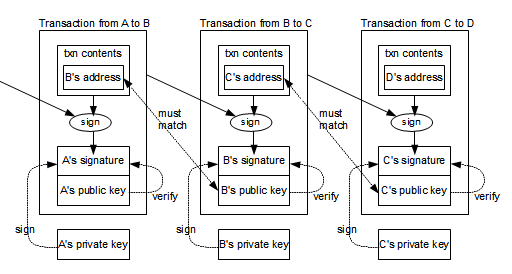
\includegraphics[scale=0.55]{bitcoindesign.png}
If we where to represent a bitcoin as a design pattern like the above and included the first transaction of a bitcoin from the address that generated the value all the way to the most recent exchange from the previous address to the current address would be a good representation of what a bitcoin looks like. Representing value in this digital record approach appeals to many as it doesn't require overhead administration  to work along with no enforcing of policy's or rules of use by an administrator. There is no physical copy of the value meaning it is a lot harder to steal or go missing, it also does not take up space in the physical world. No validating of the exchange by a 3rd party or outside source means transactions can be a lot faster compared to there fiat counterpart. The autonomous method for creating bitcoins at a set rate until a certain amount exist gives a scarcity and value to the coin as more cannot be printed.

\subsection{Blockchain: What is the blockchain?}
The block-chain is a design pattern that came about with the creation of bitcoin, this design pattern solved a problem that plagued computer scientists during the early years of the internet. The problem was how can we have people exchange services and things of value on the internet without a middleman or overseeing power having to get involved. The blockchain works by combining the collective processing power of computer systems worldwide in order to process transactions. These machines vary from high performance computers to groups of less effective computers known as mining pools. About every 10 minutes these computers, also known to the cryptocurrancy community as "miners" will collect a bunch of pending transactions and create a unsolved block. To solve the block we take the address of the previous block and combine it with a nonce which is provided by the miner’s CPU power, this this is just a newly generated hash similar to the one from the previous block. Saoshi mentions in the published paper that the two hash strings are used in a series of calculations based on Adam Back's Hashcash, a algorithm created to stop denial-of-service attacks using cryptographic hashes such as SHA1, SHA256 or SHA3. The hash that is taken as the solution is the first miner to produce a SHA256 hash that has a header starting with a specified number of 0’s set by the block-chains difficulty.  The block-chain difficulty fluctuates depending on the rate of blocks being produced. Below is a simplified representation of what the blockchain looks like.
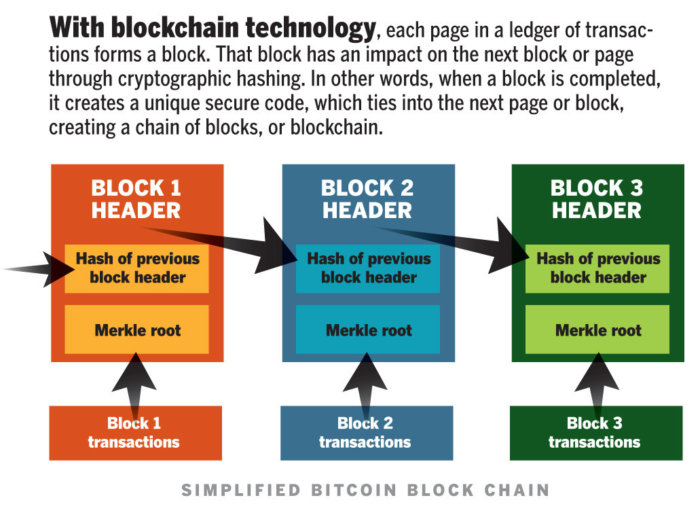
\includegraphics[scale=0.5]{blockchaindesign.jpg}
\subsection{Applications interactions with the blockchain: API's}
\textbf{Blockchain.info:} This is a website that can be used to examine transactions and blocks that have been validated on the blockchain. You can also use this site to create an online wallet for storing your own bitcoins. You can apply for an API which will grant you the ability to integrate the blockchain into your application allowing you to create a wallet, send and receive bitcoins and get information on transactions. The API uses POST and GET calls to return JSON to the application which can be then used. \break
\textbf{BlockCypher:} This is another API that returns JSON to the application. BlockCypher is for interacting with blockchains, accessed over HTTP or HTTPS from the api.blockcypher.com domain. One of the major pros of using this service is that it does not only offer just the bitcoin blockchain but also Ethereum, Litecoin and Dogecoin. \break
\textbf{Coinbase API:} This API is offered by the one of the most popular exchanges coinbase. This is a well established site with an API that allows you to create wallets along with sending and receiving bitcoin. This API allows you to add widgets to your application allowing users to buy bitcoin.

\section{Social Media Research}

Social media plays a crucial part in our everyday lives. Whether we like to give it that much importance it is the most prominent and hugely influential factors in our world right now. Whole business have been set up and run off the back off these social media platforms, with new revenue streams being offered thanks to their existence. More and more each day people are dependant on social media for their news instead of news outlets which then informs the users views on certain topics and products. A products reception on the social media giants like Twitter or Facebook can be make or break. A couple bad tweets, posts on Facebook or rants on YouTube can result in PR nightmares for companies and loss in revenue and stock. Social media can also be used to document users trends and habits giving vital information on what the user wants to see and where the platform is heading. 
Facebook and Twitters ability to document users information and habits has helped them stay on top and stick with whats trending and not fall by the way side like many other social media platforms. This also leads to targeted advertisements a users search history and likes and viewings are used to inform what else they will see on a platform. For example a common thing you may have come across is: you have searched or liked something relating to a particular television show then you open up Instagram and scroll and the first advert that pops up is merchandise relating to that television show. This happens every day and with social media AI being trained to handle your own social sphere better and better your platform and overall experience can wind up completely different to those around you. 

So taking of this into account and to bring a educational crypto-currency platform to the market it is necessary to research the information and trends out there in the market and on social media. As discussed previously Social Media influences the market. Public opinion will influence the success of your product and in this day and age social media is public opinion. To Launch any sort of app these days, there Has to be some sort of social media interaction or built in functionality. Every app these days lets you follow your friends and informs you what they are doing. Each app has a communication/messaging service between its users. FAQ services and support between the user and the developer is of the up most importance a lot of this is done through social media. Take air line's social medias often people can complain to these accounts and the issues will instantly be resolved. No company wants a negative image on social media as they know people will be swayed. 

Public opinion on the topic that informs the app or the platform is based on is also hugely important. Taking this into account we can't just observe how our platform is interacts with social media and what people say about it on social media. We in fact have to look at the subject matter of our application, Bitcoin a violate crypto currency that everyone in the past year has an opinion on and has been talking about. Social media can literally affect the price of any crypto currency. From celebrities and social media personalities talking about and announcing their support or investment into a currency to people talking about the negative affects or downside of Crypto-Currencies. Bitcoin and Crypto-Currencies are a new wave and almost controversial topic. The information is out there but people aren't very well informed on the topic. With differing opinions and news flooding in on social media platforms it gets very confusing for the average person to know who to listen to and what to follow..
\section{Platform Design}

As a group Conor, Donal and I(Stephen) met regularly each week and our first plan of action was to divide the work and objectives between the 3 of us. I offered to take on some of the front end and the primary load of the aesthetics/ overall look of the project. I had previous experience in graphic design so I photo-shopped mock designs and thumbnails for the project as we went on. I familiarized myself with how the mean stack controlled its colour scheme and look through bootstrap, CSS and HTML components. I researched a lot of different style-sheets and components to make the projects UI(user interface) stand out and be intuitive. I had working design in my head that I wanted to achieve, along with receiving creative input form Conor and Donal. 

I started with the aesthetic of the home page first. Making a 2 by 2 grid with 4 thumbnails that linked to different components of the project. To make this grid and to centre it I used a CSS sheet for the home component HTML page. I wanted each of these thumbnails highlight when hovered on and portray exactly what they linked to. To do so I used Adobe Photoshop for editing and graphic design. For inspiration and templates/base images I used Google images with key words to find exactly what I was looking for. I looked at various crypto-currencies wallets, stock websites and angular apps to get a feel for how this project should look. I want to take the best aspects from each and improve on areas where I felt these other platforms could have. 

Conor informed me about Google fonts. Google fonts is a font hub offered by Google offering a free download of a endless amount of varying fonts. I browsed through the website and found multiple fonts I felt would fit the idea for the look of the app. 
My criteria for picking a font was

\begin{itemize}
\item Readability. 
\item Aesthetic Appeal.
\item Uniqueness. 
\item Topic Appropriate
\end{itemize}
when I had chosen the appropriate fonts for the appropriate sections. I started to then use bootstrap to customize pages further. The bootstrap API offers a huge library of amazingly intuitive and user friendly styling components and features. For our FAQ(Frequently Asked Questions) page I used a bootstrap comment section template for taking users comments and any questions they had about our product. 

% needed in second column of first page if using \IEEEpubid
%\IEEEpubidadjcol

% An example of a floating figure using the graphicx package.
% Note that \label must occur AFTER (or within) \caption.
% For figures, \caption should occur after the \includegraphics.
% Note that IEEEtran v1.7 and later has special internal code that
% is designed to preserve the operation of \label within \caption
% even when the captionsoff option is in effect. However, because
% of issues like this, it may be the safest practice to put all your
% \label just after \caption rather than within \caption{}.
%
% Reminder: the "draftcls" or "draftclsnofoot", not "draft", class
% option should be used if it is desired that the figures are to be
% displayed while in draft mode.
%
%\begin{figure}[!t]
%\centering
%\includegraphics[width=2.5in]{myfigure}
% where an .eps filename suffix will be assumed under latex, 
% and a .pdf suffix will be assumed for pdflatex; or what has been declared
% via \DeclareGraphicsExtensions.
%\caption{Simulation Results}
%\label{fig_sim}
%\end{figure}

% Note that IEEE typically puts floats only at the top, even when this
% results in a large percentage of a column being occupied by floats.


% An example of a double column floating figure using two subfigures.
% (The subfig.sty package must be loaded for this to work.)
% The subfigure \label commands are set within each subfloat command, the
% \label for the overall figure must come after \caption.
% \hfil must be used as a separator to get equal spacing.
% The subfigure.sty package works much the same way, except \subfigure is
% used instead of \subfloat.
%
%\begin{figure*}[!t]
%\centerline{\subfloat[Case I]\includegraphics[width=2.5in]{subfigcase1}%
%\label{fig_first_case}}
%\hfil
%\subfloat[Case II]{\includegraphics[width=2.5in]{subfigcase2}%
%\label{fig_second_case}}}
%\caption{Simulation results}
%\label{fig_sim}
%\end{figure*}
%
% Note that often IEEE papers with subfigures do not employ subfigure
% captions (using the optional argument to \subfloat), but instead will
% reference/describe all of them (a), (b), etc., within the main caption.


% An example of a floating table. Note that, for IEEE style tables, the 
% \caption command should come BEFORE the table. Table text will default to
% \footnotesize as IEEE normally uses this smaller font for tables.
% The \label must come after \caption as always.
%
%\begin{table}[!t]
%% increase table row spacing, adjust to taste
%\renewcommand{\arraystretch}{1.3}
% if using array.sty, it might be a good idea to tweak the value of
% \extrarowheight as needed to properly center the text within the cells
%\caption{An Example of a Table}
%\label{table_example}
%\centering
%% Some packages, such as MDW tools, offer better commands for making tables
%% than the plain LaTeX2e tabular which is used here.
%\begin{tabular}{|c||c|}
%\hline
%One & Two\\
%\hline
%Three & Four\\
%\hline
%\end{tabular}
%\end{table}


% Note that IEEE does not put floats in the very first column - or typically
% anywhere on the first page for that matter. Also, in-text middle ("here")
% positioning is not used. Most IEEE journals use top floats exclusively.
% Note that, LaTeX2e, unlike IEEE journals, places footnotes above bottom
% floats. This can be corrected via the \fnbelowfloat command of the
% stfloats package.



\section{Conclusion}
Todo!!




% if have a single appendix:
%\appendix[Proof of the Zonklar Equations]
% or
%\appendix  % for no appendix heading
% do not use \section anymore after \appendix, only \section*
% is possibly needed

% use appendices with more than one appendix
% then use \section to start each appendix
% you must declare a \section before using any
% \subsection or using \label (\appendices by itself
% starts a section numbered zero.)
%


\appendices
\section{Proof of the First Zonklar Equation}
Some text for the appendix.

% use section* for acknowledgement
\section*{Acknowledgment}


The authors would like to thank...


% Can use something like this to put references on a page
% by themselves when using endfloat and the captionsoff option.
\ifCLASSOPTIONcaptionsoff
  \newpage
\fi



% trigger a \newpage just before the given reference
% number - used to balance the columns on the last page
% adjust value as needed - may need to be readjusted if
% the document is modified later
%\IEEEtriggeratref{8}
% The "triggered" command can be changed if desired:
%\IEEEtriggercmd{\enlargethispage{-5in}}

% references section

% can use a bibliography generated by BibTeX as a .bbl file
% BibTeX documentation can be easily obtained at:
% http://www.ctan.org/tex-archive/biblio/bibtex/contrib/doc/
% The IEEEtran BibTeX style support page is at:
% http://www.michaelshell.org/tex/ieeetran/bibtex/
%\bibliographystyle{IEEEtran}
% argument is your BibTeX string definitions and bibliography database(s)
%\bibliography{IEEEabrv,../bib/paper}
%
% <OR> manually copy in the resultant .bbl file
% set second argument of \begin to the number of references
% (used to reserve space for the reference number labels box)
\begin{thebibliography}{1}

\bibitem{IEEEhowto:kopka}
H.~Kopka and P.~W. Daly, \emph{A Guide to \LaTeX}, 3rd~ed.\hskip 1em plus
  0.5em minus 0.4em\relax Harlow, England: Addison-Wesley, 1999.

\end{thebibliography}

% biography section
% 
% If you have an EPS/PDF photo (graphicx package needed) extra braces are
% needed around the contents of the optional argument to biography to prevent
% the LaTeX parser from getting confused when it sees the complicated
% \includegraphics command within an optional argument. (You could create
% your own custom macro containing the \includegraphics command to make things
% simpler here.)
%\begin{biography}[{\includegraphics[width=1in,height=1.25in,clip,keepaspectratio]{mshell}}]{Michael Shell}
% or if you just want to reserve a space for a photo:



% You can push biographies down or up by placing
% a \vfill before or after them. The appropriate
% use of \vfill depends on what kind of text is
% on the last page and whether or not the columns
% are being equalized.

%\vfill

% Can be used to pull up biographies so that the bottom of the last one
% is flush with the other column.
%\enlargethispage{-5in}



% that's all folks
\end{document}


